%%-------------------------------------------------------
%% AtlasAutoware: real-time on-vehicle neural network inference (Senior Research report)
%% Same skeleton as the Senior Research Report template
%% (12pt article, biblatex/biber, listings).
%%-------------------------------------------------------
\documentclass[12pt]{article}
\usepackage{float}
\usepackage{placeins}
\usepackage{graphicx}
\usepackage{subfig}
\usepackage[a4paper, portrait, margin=1in]{geometry}
\usepackage[T1]{fontenc}
\usepackage[utf8]{inputenc}
\usepackage{textcomp}
\usepackage{booktabs}
\usepackage{array}
\usepackage{hyperref}
\hypersetup{colorlinks=true, linkcolor=black, citecolor=black, urlcolor=blue!50!black}

\usepackage[font=small,labelfont=bf]{caption}
\captionsetup[figure]{font={sf, footnotesize},labelfont={sf, footnotesize}}

% Overleaf (and any full TeX Live) has biblatex; fall back to natbib/bibtex elsewhere.
\IfFileExists{biblatex.sty}{
  \usepackage[backend=biber]{biblatex}
  \addbibresource{citations.bib}
  \newcommand{\printrefs}{\printbibliography[title={References}]}
}{
  \usepackage[numbers]{natbib}
  \usepackage{url}
  \newcommand{\printrefs}{\renewcommand{\refname}{References}\bibliographystyle{plainnat}\bibliography{citations}}
}

\usepackage{listings}
\usepackage{xcolor}
\definecolor{codegreen}{rgb}{0,0.6,0}
\definecolor{codegray}{rgb}{0.5,0.5,0.5}
\definecolor{codepurple}{rgb}{0.58,0,0.82}
\definecolor{backcolour}{rgb}{0.95,0.95,0.92}
\lstdefinestyle{mystyle}{
    backgroundcolor=\color{backcolour},
    commentstyle=\color{codegreen},
    keywordstyle=\color{magenta},
    numberstyle=\tiny\color{codegray},
    stringstyle=\color{codepurple},
    basicstyle=\ttfamily\footnotesize,
    breakatwhitespace=false,
    breaklines=true,
    captionpos=b,
    keepspaces=true,
    numbers=left,
    numbersep=5pt,
    showspaces=false,
    showstringspaces=false,
    showtabs=false,
    tabsize=2
}
\lstset{style=mystyle}
\graphicspath{{figures/}{figures_report/}{results/}}
\newcommand{\resBaseNomSucc}{0.7}
\newcommand{\resBaseNomSuccLo}{0.0}
\newcommand{\resBaseNomSuccHi}{2.0}
\newcommand{\resBaseNomSuccSd}{0.0}
\newcommand{\resBaseNomColl}{83.3}
\newcommand{\resBaseNomProg}{34.5}
\newcommand{\resBaseNomUnseen}{0.0}
\newcommand{\resBaseNomUnseenProg}{27.2}
\newcommand{\resBaseLidSucc}{0.7}
\newcommand{\resBaseLidSuccLo}{0.0}
\newcommand{\resBaseLidSuccHi}{2.0}
\newcommand{\resBaseLidSuccSd}{0.0}
\newcommand{\resBaseLidColl}{81.3}
\newcommand{\resBaseLidProg}{36.2}
\newcommand{\resBaseLidUnseen}{0.0}
\newcommand{\resBaseLidUnseenProg}{29.9}
\newcommand{\resBaseCamSucc}{0.0}
\newcommand{\resBaseCamSuccLo}{0.0}
\newcommand{\resBaseCamSuccHi}{0.0}
\newcommand{\resBaseCamSuccSd}{0.0}
\newcommand{\resBaseCamColl}{70.0}
\newcommand{\resBaseCamProg}{33.3}
\newcommand{\resBaseCamUnseen}{0.0}
\newcommand{\resBaseCamUnseenProg}{31.4}
\newcommand{\resBaseNocamSucc}{0.0}
\newcommand{\resBaseNocamSuccLo}{0.0}
\newcommand{\resBaseNocamSuccHi}{0.0}
\newcommand{\resBaseNocamSuccSd}{0.0}
\newcommand{\resBaseNocamColl}{49.3}
\newcommand{\resBaseNocamProg}{20.7}
\newcommand{\resBaseNocamUnseen}{0.0}
\newcommand{\resBaseNocamUnseenProg}{23.4}
\newcommand{\resBcNomSucc}{10.2}
\newcommand{\resBcNomSuccLo}{7.5}
\newcommand{\resBcNomSuccHi}{13.1}
\newcommand{\resBcNomSuccSd}{4.4}
\newcommand{\resBcNomColl}{60.7}
\newcommand{\resBcNomProg}{67.0}
\newcommand{\resBcNomUnseen}{8.9}
\newcommand{\resBcNomUnseenProg}{56.5}
\newcommand{\resBcaugNomSucc}{4.4}
\newcommand{\resBcaugNomSuccLo}{2.7}
\newcommand{\resBcaugNomSuccHi}{6.4}
\newcommand{\resBcaugNomSuccSd}{0.8}
\newcommand{\resBcaugNomColl}{81.1}
\newcommand{\resBcaugNomProg}{63.2}
\newcommand{\resBcaugNomUnseen}{1.1}
\newcommand{\resBcaugNomUnseenProg}{48.7}
\newcommand{\resBcaugNocamSucc}{2.4}
\newcommand{\resBcaugNocamSuccLo}{1.1}
\newcommand{\resBcaugNocamSuccHi}{3.8}
\newcommand{\resBcaugNocamSuccSd}{0.6}
\newcommand{\resBcaugNocamColl}{85.6}
\newcommand{\resBcaugNocamProg}{60.4}
\newcommand{\resBcaugNocamUnseen}{0.0}
\newcommand{\resBcaugNocamUnseenProg}{50.9}
\newcommand{\resDgoneNomSucc}{4.0}
\newcommand{\resDgoneNomSuccLo}{2.2}
\newcommand{\resDgoneNomSuccHi}{5.8}
\newcommand{\resDgoneNomSuccSd}{2.2}
\newcommand{\resDgoneNomColl}{78.9}
\newcommand{\resDgoneNomProg}{60.6}
\newcommand{\resDgoneNomUnseen}{2.2}
\newcommand{\resDgoneNomUnseenProg}{45.1}
\newcommand{\resDgtwoNomSucc}{2.9}
\newcommand{\resDgtwoNomSuccLo}{1.3}
\newcommand{\resDgtwoNomSuccHi}{4.7}
\newcommand{\resDgtwoNomSuccSd}{0.8}
\newcommand{\resDgtwoNomColl}{78.0}
\newcommand{\resDgtwoNomProg}{61.1}
\newcommand{\resDgtwoNomUnseen}{0.0}
\newcommand{\resDgtwoNomUnseenProg}{44.7}
\newcommand{\resDgthreeNomSucc}{5.3}
\newcommand{\resDgthreeNomSuccLo}{3.3}
\newcommand{\resDgthreeNomSuccHi}{7.6}
\newcommand{\resDgthreeNomSuccSd}{2.8}
\newcommand{\resDgthreeNomColl}{71.3}
\newcommand{\resDgthreeNomProg}{62.6}
\newcommand{\resDgthreeNomUnseen}{0.0}
\newcommand{\resDgthreeNomUnseenProg}{49.7}
\newcommand{\resDgthreeLidSucc}{4.7}
\newcommand{\resDgthreeLidSuccLo}{2.7}
\newcommand{\resDgthreeLidSuccHi}{6.7}
\newcommand{\resDgthreeLidSuccSd}{1.4}
\newcommand{\resDgthreeLidColl}{72.0}
\newcommand{\resDgthreeLidProg}{64.0}
\newcommand{\resDgthreeLidUnseen}{0.0}
\newcommand{\resDgthreeLidUnseenProg}{52.1}
\newcommand{\resDgthreeCamSucc}{3.8}
\newcommand{\resDgthreeCamSuccLo}{2.2}
\newcommand{\resDgthreeCamSuccHi}{5.6}
\newcommand{\resDgthreeCamSuccSd}{0.8}
\newcommand{\resDgthreeCamColl}{71.8}
\newcommand{\resDgthreeCamProg}{63.2}
\newcommand{\resDgthreeCamUnseen}{0.0}
\newcommand{\resDgthreeCamUnseenProg}{49.9}
\newcommand{\resDgthreeNocamSucc}{2.7}
\newcommand{\resDgthreeNocamSuccLo}{1.3}
\newcommand{\resDgthreeNocamSuccHi}{4.2}
\newcommand{\resDgthreeNocamSuccSd}{0.5}
\newcommand{\resDgthreeNocamColl}{77.8}
\newcommand{\resDgthreeNocamProg}{57.2}
\newcommand{\resDgthreeNocamUnseen}{1.1}
\newcommand{\resDgthreeNocamUnseenProg}{44.8}
\newcommand{\resAbllidNomSucc}{2.0}
\newcommand{\resAbllidNomSuccLo}{0.0}
\newcommand{\resAbllidNomSuccHi}{4.7}
\newcommand{\resAbllidNomSuccSd}{0.0}
\newcommand{\resAbllidNomColl}{83.3}
\newcommand{\resAbllidNomProg}{62.7}
\newcommand{\resAbllidNomUnseen}{0.0}
\newcommand{\resAbllidNomUnseenProg}{56.6}
\newcommand{\resAblcamNomSucc}{3.3}
\newcommand{\resAblcamNomSuccLo}{0.7}
\newcommand{\resAblcamNomSuccHi}{6.7}
\newcommand{\resAblcamNomSuccSd}{0.0}
\newcommand{\resAblcamNomColl}{76.0}
\newcommand{\resAblcamNomProg}{70.5}
\newcommand{\resAblcamNomUnseen}{0.0}
\newcommand{\resAblcamNomUnseenProg}{52.5}
% generated by ml/summarize_results.py -- do not edit
\providecommand{\resBaseNomSucc}{n/a}
\providecommand{\resBaseNomSuccLo}{n/a}
\providecommand{\resBaseNomSuccHi}{n/a}
\providecommand{\resBaseNomSuccSd}{n/a}
\providecommand{\resBaseNomColl}{n/a}
\providecommand{\resBaseNomProg}{n/a}
\providecommand{\resBaseNomUnseen}{n/a}
\providecommand{\resBaseNomUnseenProg}{n/a}
\providecommand{\resBaseLidSucc}{n/a}
\providecommand{\resBaseLidSuccLo}{n/a}
\providecommand{\resBaseLidSuccHi}{n/a}
\providecommand{\resBaseLidSuccSd}{n/a}
\providecommand{\resBaseLidColl}{n/a}
\providecommand{\resBaseLidProg}{n/a}
\providecommand{\resBaseLidUnseen}{n/a}
\providecommand{\resBaseLidUnseenProg}{n/a}
\providecommand{\resBaseCamSucc}{n/a}
\providecommand{\resBaseCamSuccLo}{n/a}
\providecommand{\resBaseCamSuccHi}{n/a}
\providecommand{\resBaseCamSuccSd}{n/a}
\providecommand{\resBaseCamColl}{n/a}
\providecommand{\resBaseCamProg}{n/a}
\providecommand{\resBaseCamUnseen}{n/a}
\providecommand{\resBaseCamUnseenProg}{n/a}
\providecommand{\resBaseNocamSucc}{n/a}
\providecommand{\resBaseNocamSuccLo}{n/a}
\providecommand{\resBaseNocamSuccHi}{n/a}
\providecommand{\resBaseNocamSuccSd}{n/a}
\providecommand{\resBaseNocamColl}{n/a}
\providecommand{\resBaseNocamProg}{n/a}
\providecommand{\resBaseNocamUnseen}{n/a}
\providecommand{\resBaseNocamUnseenProg}{n/a}
\providecommand{\resBcNomSucc}{n/a}
\providecommand{\resBcNomSuccLo}{n/a}
\providecommand{\resBcNomSuccHi}{n/a}
\providecommand{\resBcNomSuccSd}{n/a}
\providecommand{\resBcNomColl}{n/a}
\providecommand{\resBcNomProg}{n/a}
\providecommand{\resBcNomUnseen}{n/a}
\providecommand{\resBcNomUnseenProg}{n/a}
\providecommand{\resBcLidSucc}{n/a}
\providecommand{\resBcLidSuccLo}{n/a}
\providecommand{\resBcLidSuccHi}{n/a}
\providecommand{\resBcLidSuccSd}{n/a}
\providecommand{\resBcLidColl}{n/a}
\providecommand{\resBcLidProg}{n/a}
\providecommand{\resBcLidUnseen}{n/a}
\providecommand{\resBcLidUnseenProg}{n/a}
\providecommand{\resBcCamSucc}{n/a}
\providecommand{\resBcCamSuccLo}{n/a}
\providecommand{\resBcCamSuccHi}{n/a}
\providecommand{\resBcCamSuccSd}{n/a}
\providecommand{\resBcCamColl}{n/a}
\providecommand{\resBcCamProg}{n/a}
\providecommand{\resBcCamUnseen}{n/a}
\providecommand{\resBcCamUnseenProg}{n/a}
\providecommand{\resBcNocamSucc}{n/a}
\providecommand{\resBcNocamSuccLo}{n/a}
\providecommand{\resBcNocamSuccHi}{n/a}
\providecommand{\resBcNocamSuccSd}{n/a}
\providecommand{\resBcNocamColl}{n/a}
\providecommand{\resBcNocamProg}{n/a}
\providecommand{\resBcNocamUnseen}{n/a}
\providecommand{\resBcNocamUnseenProg}{n/a}
\providecommand{\resBcaugNomSucc}{n/a}
\providecommand{\resBcaugNomSuccLo}{n/a}
\providecommand{\resBcaugNomSuccHi}{n/a}
\providecommand{\resBcaugNomSuccSd}{n/a}
\providecommand{\resBcaugNomColl}{n/a}
\providecommand{\resBcaugNomProg}{n/a}
\providecommand{\resBcaugNomUnseen}{n/a}
\providecommand{\resBcaugNomUnseenProg}{n/a}
\providecommand{\resBcaugLidSucc}{n/a}
\providecommand{\resBcaugLidSuccLo}{n/a}
\providecommand{\resBcaugLidSuccHi}{n/a}
\providecommand{\resBcaugLidSuccSd}{n/a}
\providecommand{\resBcaugLidColl}{n/a}
\providecommand{\resBcaugLidProg}{n/a}
\providecommand{\resBcaugLidUnseen}{n/a}
\providecommand{\resBcaugLidUnseenProg}{n/a}
\providecommand{\resBcaugCamSucc}{n/a}
\providecommand{\resBcaugCamSuccLo}{n/a}
\providecommand{\resBcaugCamSuccHi}{n/a}
\providecommand{\resBcaugCamSuccSd}{n/a}
\providecommand{\resBcaugCamColl}{n/a}
\providecommand{\resBcaugCamProg}{n/a}
\providecommand{\resBcaugCamUnseen}{n/a}
\providecommand{\resBcaugCamUnseenProg}{n/a}
\providecommand{\resBcaugNocamSucc}{n/a}
\providecommand{\resBcaugNocamSuccLo}{n/a}
\providecommand{\resBcaugNocamSuccHi}{n/a}
\providecommand{\resBcaugNocamSuccSd}{n/a}
\providecommand{\resBcaugNocamColl}{n/a}
\providecommand{\resBcaugNocamProg}{n/a}
\providecommand{\resBcaugNocamUnseen}{n/a}
\providecommand{\resBcaugNocamUnseenProg}{n/a}
\providecommand{\resDgoneNomSucc}{n/a}
\providecommand{\resDgoneNomSuccLo}{n/a}
\providecommand{\resDgoneNomSuccHi}{n/a}
\providecommand{\resDgoneNomSuccSd}{n/a}
\providecommand{\resDgoneNomColl}{n/a}
\providecommand{\resDgoneNomProg}{n/a}
\providecommand{\resDgoneNomUnseen}{n/a}
\providecommand{\resDgoneNomUnseenProg}{n/a}
\providecommand{\resDgoneLidSucc}{n/a}
\providecommand{\resDgoneLidSuccLo}{n/a}
\providecommand{\resDgoneLidSuccHi}{n/a}
\providecommand{\resDgoneLidSuccSd}{n/a}
\providecommand{\resDgoneLidColl}{n/a}
\providecommand{\resDgoneLidProg}{n/a}
\providecommand{\resDgoneLidUnseen}{n/a}
\providecommand{\resDgoneLidUnseenProg}{n/a}
\providecommand{\resDgoneCamSucc}{n/a}
\providecommand{\resDgoneCamSuccLo}{n/a}
\providecommand{\resDgoneCamSuccHi}{n/a}
\providecommand{\resDgoneCamSuccSd}{n/a}
\providecommand{\resDgoneCamColl}{n/a}
\providecommand{\resDgoneCamProg}{n/a}
\providecommand{\resDgoneCamUnseen}{n/a}
\providecommand{\resDgoneCamUnseenProg}{n/a}
\providecommand{\resDgoneNocamSucc}{n/a}
\providecommand{\resDgoneNocamSuccLo}{n/a}
\providecommand{\resDgoneNocamSuccHi}{n/a}
\providecommand{\resDgoneNocamSuccSd}{n/a}
\providecommand{\resDgoneNocamColl}{n/a}
\providecommand{\resDgoneNocamProg}{n/a}
\providecommand{\resDgoneNocamUnseen}{n/a}
\providecommand{\resDgoneNocamUnseenProg}{n/a}
\providecommand{\resDgtwoNomSucc}{n/a}
\providecommand{\resDgtwoNomSuccLo}{n/a}
\providecommand{\resDgtwoNomSuccHi}{n/a}
\providecommand{\resDgtwoNomSuccSd}{n/a}
\providecommand{\resDgtwoNomColl}{n/a}
\providecommand{\resDgtwoNomProg}{n/a}
\providecommand{\resDgtwoNomUnseen}{n/a}
\providecommand{\resDgtwoNomUnseenProg}{n/a}
\providecommand{\resDgtwoLidSucc}{n/a}
\providecommand{\resDgtwoLidSuccLo}{n/a}
\providecommand{\resDgtwoLidSuccHi}{n/a}
\providecommand{\resDgtwoLidSuccSd}{n/a}
\providecommand{\resDgtwoLidColl}{n/a}
\providecommand{\resDgtwoLidProg}{n/a}
\providecommand{\resDgtwoLidUnseen}{n/a}
\providecommand{\resDgtwoLidUnseenProg}{n/a}
\providecommand{\resDgtwoCamSucc}{n/a}
\providecommand{\resDgtwoCamSuccLo}{n/a}
\providecommand{\resDgtwoCamSuccHi}{n/a}
\providecommand{\resDgtwoCamSuccSd}{n/a}
\providecommand{\resDgtwoCamColl}{n/a}
\providecommand{\resDgtwoCamProg}{n/a}
\providecommand{\resDgtwoCamUnseen}{n/a}
\providecommand{\resDgtwoCamUnseenProg}{n/a}
\providecommand{\resDgtwoNocamSucc}{n/a}
\providecommand{\resDgtwoNocamSuccLo}{n/a}
\providecommand{\resDgtwoNocamSuccHi}{n/a}
\providecommand{\resDgtwoNocamSuccSd}{n/a}
\providecommand{\resDgtwoNocamColl}{n/a}
\providecommand{\resDgtwoNocamProg}{n/a}
\providecommand{\resDgtwoNocamUnseen}{n/a}
\providecommand{\resDgtwoNocamUnseenProg}{n/a}
\providecommand{\resDgthreeNomSucc}{n/a}
\providecommand{\resDgthreeNomSuccLo}{n/a}
\providecommand{\resDgthreeNomSuccHi}{n/a}
\providecommand{\resDgthreeNomSuccSd}{n/a}
\providecommand{\resDgthreeNomColl}{n/a}
\providecommand{\resDgthreeNomProg}{n/a}
\providecommand{\resDgthreeNomUnseen}{n/a}
\providecommand{\resDgthreeNomUnseenProg}{n/a}
\providecommand{\resDgthreeLidSucc}{n/a}
\providecommand{\resDgthreeLidSuccLo}{n/a}
\providecommand{\resDgthreeLidSuccHi}{n/a}
\providecommand{\resDgthreeLidSuccSd}{n/a}
\providecommand{\resDgthreeLidColl}{n/a}
\providecommand{\resDgthreeLidProg}{n/a}
\providecommand{\resDgthreeLidUnseen}{n/a}
\providecommand{\resDgthreeLidUnseenProg}{n/a}
\providecommand{\resDgthreeCamSucc}{n/a}
\providecommand{\resDgthreeCamSuccLo}{n/a}
\providecommand{\resDgthreeCamSuccHi}{n/a}
\providecommand{\resDgthreeCamSuccSd}{n/a}
\providecommand{\resDgthreeCamColl}{n/a}
\providecommand{\resDgthreeCamProg}{n/a}
\providecommand{\resDgthreeCamUnseen}{n/a}
\providecommand{\resDgthreeCamUnseenProg}{n/a}
\providecommand{\resDgthreeNocamSucc}{n/a}
\providecommand{\resDgthreeNocamSuccLo}{n/a}
\providecommand{\resDgthreeNocamSuccHi}{n/a}
\providecommand{\resDgthreeNocamSuccSd}{n/a}
\providecommand{\resDgthreeNocamColl}{n/a}
\providecommand{\resDgthreeNocamProg}{n/a}
\providecommand{\resDgthreeNocamUnseen}{n/a}
\providecommand{\resDgthreeNocamUnseenProg}{n/a}
\providecommand{\resAbllidNomSucc}{n/a}
\providecommand{\resAbllidNomSuccLo}{n/a}
\providecommand{\resAbllidNomSuccHi}{n/a}
\providecommand{\resAbllidNomSuccSd}{n/a}
\providecommand{\resAbllidNomColl}{n/a}
\providecommand{\resAbllidNomProg}{n/a}
\providecommand{\resAbllidNomUnseen}{n/a}
\providecommand{\resAbllidNomUnseenProg}{n/a}
\providecommand{\resAbllidLidSucc}{n/a}
\providecommand{\resAbllidLidSuccLo}{n/a}
\providecommand{\resAbllidLidSuccHi}{n/a}
\providecommand{\resAbllidLidSuccSd}{n/a}
\providecommand{\resAbllidLidColl}{n/a}
\providecommand{\resAbllidLidProg}{n/a}
\providecommand{\resAbllidLidUnseen}{n/a}
\providecommand{\resAbllidLidUnseenProg}{n/a}
\providecommand{\resAbllidCamSucc}{n/a}
\providecommand{\resAbllidCamSuccLo}{n/a}
\providecommand{\resAbllidCamSuccHi}{n/a}
\providecommand{\resAbllidCamSuccSd}{n/a}
\providecommand{\resAbllidCamColl}{n/a}
\providecommand{\resAbllidCamProg}{n/a}
\providecommand{\resAbllidCamUnseen}{n/a}
\providecommand{\resAbllidCamUnseenProg}{n/a}
\providecommand{\resAbllidNocamSucc}{n/a}
\providecommand{\resAbllidNocamSuccLo}{n/a}
\providecommand{\resAbllidNocamSuccHi}{n/a}
\providecommand{\resAbllidNocamSuccSd}{n/a}
\providecommand{\resAbllidNocamColl}{n/a}
\providecommand{\resAbllidNocamProg}{n/a}
\providecommand{\resAbllidNocamUnseen}{n/a}
\providecommand{\resAbllidNocamUnseenProg}{n/a}
\providecommand{\resAblcamNomSucc}{n/a}
\providecommand{\resAblcamNomSuccLo}{n/a}
\providecommand{\resAblcamNomSuccHi}{n/a}
\providecommand{\resAblcamNomSuccSd}{n/a}
\providecommand{\resAblcamNomColl}{n/a}
\providecommand{\resAblcamNomProg}{n/a}
\providecommand{\resAblcamNomUnseen}{n/a}
\providecommand{\resAblcamNomUnseenProg}{n/a}
\providecommand{\resAblcamLidSucc}{n/a}
\providecommand{\resAblcamLidSuccLo}{n/a}
\providecommand{\resAblcamLidSuccHi}{n/a}
\providecommand{\resAblcamLidSuccSd}{n/a}
\providecommand{\resAblcamLidColl}{n/a}
\providecommand{\resAblcamLidProg}{n/a}
\providecommand{\resAblcamLidUnseen}{n/a}
\providecommand{\resAblcamLidUnseenProg}{n/a}
\providecommand{\resAblcamCamSucc}{n/a}
\providecommand{\resAblcamCamSuccLo}{n/a}
\providecommand{\resAblcamCamSuccHi}{n/a}
\providecommand{\resAblcamCamSuccSd}{n/a}
\providecommand{\resAblcamCamColl}{n/a}
\providecommand{\resAblcamCamProg}{n/a}
\providecommand{\resAblcamCamUnseen}{n/a}
\providecommand{\resAblcamCamUnseenProg}{n/a}
\providecommand{\resAblcamNocamSucc}{n/a}
\providecommand{\resAblcamNocamSuccLo}{n/a}
\providecommand{\resAblcamNocamSuccHi}{n/a}
\providecommand{\resAblcamNocamSuccSd}{n/a}
\providecommand{\resAblcamNocamColl}{n/a}
\providecommand{\resAblcamNocamProg}{n/a}
\providecommand{\resAblcamNocamUnseen}{n/a}
\providecommand{\resAblcamNocamUnseenProg}{n/a}


\title{AtlasAutoware: Real-Time On-Vehicle Neural Network Inference\\
for Autonomous 1/10-Scale Racing}
\author{Eshan Iyer}
\date{\today}

\begin{document}
\maketitle

\begin{abstract}
\noindent A 1/10-scale racing car has a 100\,ms control period and one small computer. This
report describes AtlasAutoware, a Jetson Orin Nano car that runs two neural networks on board
inside that budget: a YOLOv8 opponent detector (5.4\,ms as a TensorRT FP16 engine) and a
1.46\,M-parameter goal-conditioned driving policy distilled from a planning expert (1.8\,ms on
the CPU with ONNX Runtime, 0.25\,ms in TensorRT). Most of the work is the platform that makes
on-vehicle inference meaningful: actuation with feedback, sensing in the policy's frame, a
browser teleoperation channel that doubles as a data channel, and a repository from which the
car can be rebuilt. The central finding is about deployment rather than models. An end-to-end
audit found that the car would have driven the learned policy at full steering lock and almost
zero speed, because the network's (speed, steer) output was unpacked as (steer, speed); the lidar
image it was trained on had been through lossy video compression; and the camera it expected
had been removed. A closed-loop evaluation in simulation, sharing its input code with the car,
measured the policy as deployed at 0\% goal success and 2.6\% route progress. After fixing the
interface, the data and the inertia problem, route progress rose to \resBcNomProg\% while goal
success stays low (\resDgthreeNomSucc\% after three rounds of DAgger), which is reported as
it is. The platform also runs Ubuntu~26.04 with ROS~2 Lyrical in a container, with the
package building and all unit tests passing there.
\end{abstract}

\section*{Introduction}

This project picks up the 1/10-scale self-driving car in the SysLab annex where the
2024 Senior Research work left it \cite{gagvani2024}. That report ended with a car
that could follow a hallway wall using a hobby ESC, a PWM breakout board and the
DonkeyCar library, and it recommended that the next group not deviate from the
F1TENTH bill of materials, because every substitution costs weeks.

The question this report asks is narrower than ``can a learned policy race''. It is whether
neural networks can run \emph{on the vehicle}, inside its control loop, and be trusted there:
fast enough on a 25\,W Jetson, alongside the classical stack, and with the numbers they
produce reaching the actuator with the meaning they had in training. The two networks are a
YOLOv8 car detector for head-to-head racing and a small goal-conditioned driving policy (the
``student'') distilled from a planning expert in simulation, with an optional feature-matching
term toward a driving vision-language model as teacher \cite{qwenrobot}. Large
vision-language-action models \cite{openvla, pi0, groot} do not fit this computer, so the
student is the on-board half of that idea.

A policy is only as good as the robot underneath it, and the robot I inherited could not have
produced usable training data or executed a learned command. It could not report how fast its
wheels were turning, it had no inertial measurement, it could only be driven by a person
standing next to it with a wired gamepad, and its configuration lived in one laptop. The first
half of this report is therefore about the platform, each change justified by what it makes
possible later:

\begin{enumerate}
  \item \textbf{Actuation with feedback.} Rebuild the drivetrain around the VESC motor
        controller, so commands are currents and speeds with measured consequences.
  \item \textbf{Sensing in the policy's coordinate frame.} Bring the lidar and camera into
        ROS~2 in the shape the stack expects, including the camera's inertial unit.
  \item \textbf{Teleoperation as a data channel.} Make the car drivable from a browser, so
        demonstrations can be collected by anyone, with the same message a policy emits.
  \item \textbf{Reproducibility as infrastructure.} Put configuration, firmware state and
        scripts in the repository, so a second car is a clone instead of a rebuild.
\end{enumerate}

The second half is about the networks on the car: how fast they run and what happens when
they share the computer (Section~\ref{sec:inference}), an end-to-end audit of the learned
policy's path from training data to actuator (Section~\ref{sec:audit}), and closed-loop training
and evaluation in simulation (Sections~\ref{sec:training}--\ref{sec:results}). All of it is in
the team repository \cite{atlasrepo}. What I have \emph{not} done is drive the learned policy
on the floor; every closed-loop number here is from simulation, and the Limitations section
says what that does and does not show.

\section*{Prior Approaches}

Three earlier designs shaped the choices here.

The 2024 report \cite{gagvani2024} drove the same chassis through a PCA9685 PWM
generator into an 80\,A hobby ESC. That path works with DonkeyCar and needs no motor
controller protocol, but it is open loop: the ESC reports nothing back, so there is no
wheel speed, no current, no temperature, and no way to calibrate throttle except by
driving. The report describes spending several months trying to control a VESC over USB
and through an Arduino before switching to the hobby ESC.

The F1TENTH reference stack \cite{f1tenthsystem} uses the VESC over USB with a ROS~2
driver, converts Ackermann commands into VESC RPM set-points, and reconstructs odometry
from the VESC's electrical RPM. It expects a Hokuyo lidar on Ethernet and a specific
gamepad. The Jetson in the lab already had this stack installed, but with a lidar
launch file for a sensor the car does not have and a control mode that had caused a
motor to overheat.

The team's own AtlasAutoware stack \cite{atlaspaper} contributes the planning and control
layer: a linear time-varying model predictive controller for raceline tracking with a
persistent warm-started quadratic program (0.6\,ms mean solve time in the reported
benchmark), a Model- and Acceleration-based Pursuit fallback, minimum-curvature raceline
refinement, a friction-limited velocity profile, an IMU-based traction governor,
actuation-latency compensation and a Frenet-frame overtaking planner. Those results
were obtained in the simulator against a kinematic bicycle plant. The hardware layer in
that paper assumed an OAK-D Pro camera, which is again what the car carries.

MuSHR \cite{mushr} is the other common open racecar design and uses the same VESC
interface, which is one reason to adopt it: any VESC-based stack becomes usable on this
car.

\section*{System Architecture}

\begin{figure}[H]
  \centering
  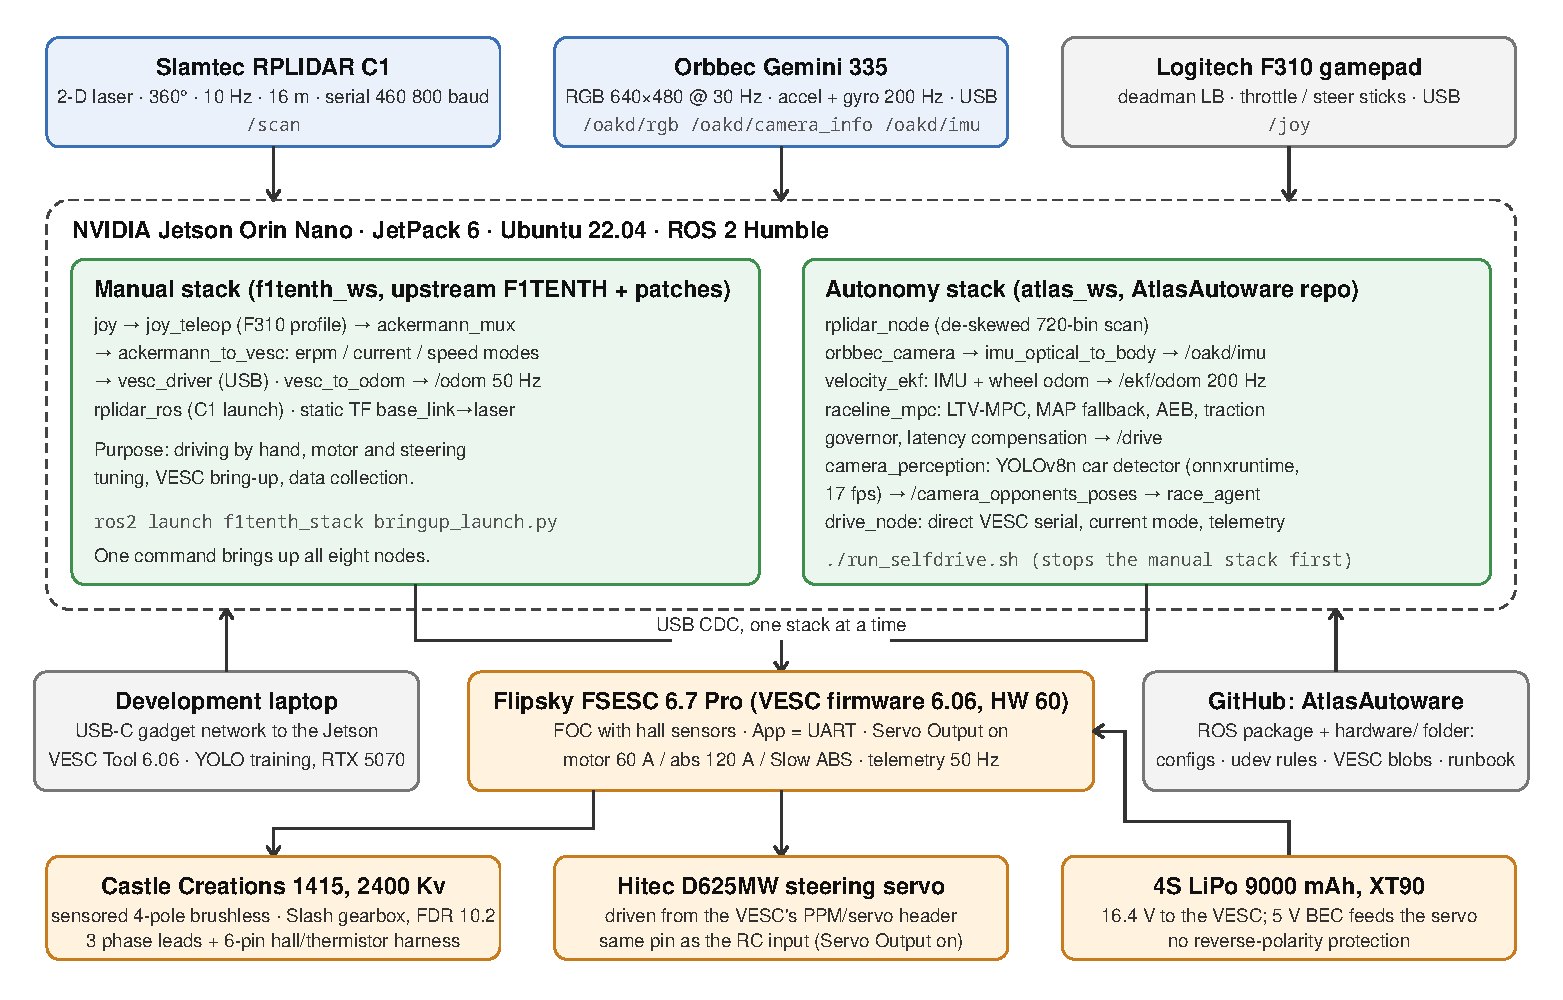
\includegraphics[width=\textwidth]{architecture.pdf}
  \caption{The car as built. Blue: sensors. Green: the two ROS~2 workspaces on the
  Jetson. Amber: the power and actuation chain. Grey: the development laptop and the
  repository. Only one workspace talks to the VESC at a time; the autonomy launcher
  stops the manual stack before it starts. Read as substrate for the pivot: the sensor
  row is the observation space, the amber chain is the action space with feedback, and
  the manual stack's teleoperation path is where a policy server later attaches
  (Figure~\ref{fig:pivot}).}
  \label{fig:arch}
\end{figure}

Figure~\ref{fig:arch} shows the system. Two ROS~2 workspaces live on the Jetson and
share the same hardware. The manual stack is the upstream F1TENTH system with our
patches: a gamepad drives the car through the F1TENTH Ackermann mux and VESC driver,
and it is what I use to tune the motor controller and to drive the car by hand. The
autonomy stack is the AtlasAutoware package. It has its own lidar node (which de-skews
each scan using the velocity estimate), its own VESC driver, the velocity EKF, the MPC
racing node and the camera perception node. The two stacks cannot both own the VESC's
USB port, so the autonomy launcher kills the manual stack before starting.

Table~\ref{tab:parts} lists the hardware. Compared with the 2024 build, the ESC, motor,
camera, lidar and battery are all different; the chassis, Jetson and servo are the same.

\begin{table}[H]
  \centering
  \small
  \begin{tabular}{p{4.3cm} p{10.2cm}}
    \toprule
    Part & Notes \\
    \midrule
    NVIDIA Jetson Orin Nano Super & JetPack 7.2.1 (L4T R39.2.1), Ubuntu 24.04, ROS~2 Jazzy,
      CUDA 13.2, TensorRT 10.16, 25\,W power mode. Reached from the laptop over the USB-C
      gadget network at 192.168.55.1. An Ubuntu 26.04 / ROS~2 Lyrical container runs beside it
      (Section~\ref{sec:lyrical}). \\
    Flipsky FSESC 6.7 Pro & VESC firmware 6.06 on the HW~60 profile. Replaced once after
      reversed battery leads destroyed the first board (the VESC has no reverse-polarity
      protection). \\
    Castle Creations 1415, 2400\,Kv & Sensored 4-pole brushless motor, 5\,mm shaft, with the
      hall/thermistor harness wired to the VESC's 6-pin sensor port. Replaced the stock
      Traxxas Velineon 3500. \\
    Traxxas Slash drivetrain & Final drive ratio 10.2, 0.109\,m tires, on a laser-cut deck. \\
    Hitec D625MW & Steering servo on the VESC's servo header. \\
    Slamtec RPLIDAR C1 & 2-D lidar, 360\textdegree{}, 10\,Hz, 16\,m, 460\,800 baud over a
      CP210x serial adapter \cite{rplidarc1}. \\
    Luxonis OAK-D Pro & RGB camera (640$\times$360 preview) with a 200\,Hz IMU, through DepthAI~2.33.
      An Orbbec Gemini 335 \cite{gemini335} was used in early September and is kept as a launch
      option. \\
    Logitech F310 & Wired gamepad, XInput mode. \\
    4S LiPo, 9000\,mAh, XT90 & 16.4\,V measured. The VESC's 5\,V BEC powers the servo. \\
    \bottomrule
  \end{tabular}
  \caption{Hardware on the car as of September 2026.}
  \label{tab:parts}
\end{table}

\section*{Stage 1: Actuation with feedback}

A demonstration is a pair: what the world looked like, and what the driver did. The
second half is worthless if ``what the driver did'' cannot be measured. The 2024 car
commanded a hobby ESC with a unitless PWM pulse and got nothing back, so its own report
notes that throttle could not be calibrated and that the same pulse produced different
speeds on different surfaces. A policy trained on those labels would be learning a
mapping that does not exist. The VESC gives the action space real units: currents and
speeds with measured consequences.

\subsection*{Getting the VESC to drive the motor}

The VESC is attractive because it closes the loop: it measures phase currents, estimates
rotor speed, exposes a PID speed controller, and reports voltage, current and
temperature over USB at 50\,Hz. It is also unforgiving. Three problems consumed most of
this stage.

The first was motor control itself. With the stock sensorless Velineon motor, the VESC's
field-oriented control depends on a back-EMF observer that has nothing to observe at
standstill. Below roughly 2000 electrical RPM the motor cogged, drew current without
moving, and twice heated its phase wires until solder joints failed. Tuning helped
(the working configuration used an observer gain of 62, a sensorless threshold of
2000 electrical RPM, motor current limits of 50--60\,A and the firmware's slow
absolute-current limit, without which current ripple tripped the over-current fault),
but the underlying dead zone was physical. I replaced the motor with a sensored Castle
1415 whose hall sensors give the controller rotor position from zero speed. Detection
with hall sensors produced a hall table and motor parameters that the firmware's
observer tracked cleanly up to the 10\,000 electrical RPM I tested on a stand.

The second was the software's response to the same dead zone. Both stacks originally
commanded the VESC in RPM mode. Someone on the team had already added a custom
\texttt{erpm} control mode to the F1TENTH \texttt{ackermann\_to\_vesc} node that never
commands below 3000 electrical RPM, and a matching \texttt{current} mode in the
AtlasAutoware \texttt{drive\_node} that maps the planner's speed to motor current with a
feed-forward minimum of 10\,A, so the car breaks stiction the instant a non-zero speed
is requested instead of waiting for the RPM loop to wind up. With a sensored motor these
are no longer necessary for safety, but current mode remains the default for the
autonomy path because it gives the MPC direct torque authority. The speed-to-RPM gain
that odometry depends on was also wrong in both stacks (it was the reference car's
value, 4614); for this drivetrain it is $60 \cdot 10.2 \cdot 2 / (\pi \cdot 0.109) \approx
3575$ electrical RPM per m/s.

The third problem is the one worth recording for whoever comes next, because it cost a
day and had no error message. After the replacement VESC was installed and configured,
the motor ran from VESC~Tool on the laptop but not from ROS: every command from the
Jetson produced zero duty, zero current and fault code zero. Rather than keep guessing
from the ROS side, I wrote a small Python implementation of the VESC serial protocol
(CRC-16/XMODEM packet framing, \texttt{COMM\_GET\_VALUES}, \texttt{COMM\_SET\_RPM},
\texttt{COMM\_GET\_MCCONF}, \texttt{COMM\_GET\_APPCONF}) and a decoder for the firmware's
serialized configuration, taking the field order and the float16 scale factors from
\texttt{confgenerator.c} in the 6.06 firmware source \cite{bldc}. That made the cause
visible in one read. A fresh Flipsky board ships with the RC-input application enabled
(\texttt{app\_to\_use = PPM\_UART}) and servo output disabled. On this hardware the
PPM input and the servo output share one pin, so the steering servo's signal wire was
being decoded as an RC receiver, and the PPM application overwrote every USB command with
``neutral'' fifty times a second. Setting \texttt{servo\_out\_enable}, switching the
application to UART and rebooting the controller fixed both the motor and the steering
at once. The same tooling then wrote the current limits (60\,A motor, 120\,A absolute,
slow absolute-current limit on) and saved the complete motor and application
configurations as binary blobs in the repository, so the next dead board can be restored
in seconds without VESC~Tool.

\subsection*{What the actuation layer now provides}

From the manual stack, the F310 gamepad drives the car with a dead-man button. From the
autonomy stack, \texttt{drive\_node} auto-detects the VESC on its stable udev path,
commands current or speed, publishes wheel-speed odometry at 20\,Hz and logs battery
voltage, MOSFET temperature and fault codes. On the bench the VESC held commanded speeds
of 1500, 3500, 6000 and 9000 electrical RPM to within 1\% at 1.5--3\,A.

\section*{Stage 2: Sensing, observations and proprioception}

A vision-language policy conditions on what the robot sees and, if it is to drive
rather than sightsee, on how the robot is moving. This stage supplies both, in the
coordinate conventions the rest of the stack (and any policy trained on its logs)
assumes.

\subsection*{Lidar}

The lidar is an RPLIDAR C1, not the A2 the launch files assumed. The C1 uses 460\,800
baud, and the A2, A3 and S1 launch files all time out on it silently. Both stacks were
changed to the C1 settings; the F1TENTH bring-up now starts the lidar itself instead of
requiring a second launch. The scan arrives at 10\,Hz with 16\,m range.

\subsection*{Camera and IMU}

The AtlasAutoware stack was written for an OAK-D Pro and consumes three topics from it:
a colour image, its calibration, and a single \texttt{sensor\_msgs/Imu} message carrying
both acceleration and angular rate. The important consumer is not vision. The
\texttt{velocity\_ekf} node fuses the IMU with wheel odometry into a 200\,Hz velocity
estimate that the lidar node uses to de-skew each 100\,ms sweep, and the MPC's traction
governor reads the gyro yaw rate to back off speed when the car slides. Without an IMU
both features are inert.

For three weeks in September the car carried an Orbbec Gemini~335 instead; it has since
gone back to the OAK-D Pro (DepthAI~2.33, 640$\times$360 at 30\,Hz with a 200\,Hz IMU), which
the launch files now select by default. The Orbbec episode is still worth recording. I replaced
the OAK-D node with the official Orbbec ROS~2 driver \cite{orbbecros2}
(OrbbecSDK v2 branch, built on the Jetson) and remapped its colour topics onto the names
the stack expects. The IMU needed more than a rename. The Orbbec reports acceleration
and angular rate in the camera's optical frame ($x$ right, $y$ down, $z$ forward),
while the EKF and the governor assume ROS body axes ($x$ forward, $z$ up)
\cite{rep103}. Fed directly, the EKF would have integrated lateral acceleration as
forward acceleration and treated roll rate as yaw rate. A 60-line relay node,
\texttt{imu\_optical\_to\_body}, rotates both vectors and their covariances. It also
publishes with reliable QoS, because the EKF subscribes with the ROS~2 default and a
best-effort publisher never matches it: the first version of the relay produced a
200\,Hz stream that nobody received, with no warning beyond one line in the log.

Building the driver exposed a JetPack quirk that will bite any C++ package using
OpenCV: the image had NVIDIA's OpenCV 4.8 development headers installed alongside
Ubuntu's 4.5.4 libraries, so every \texttt{find\_package(OpenCV)} failed. Downgrading
the development package to 4.5.4 to match the runtime fixed it. The camera negotiates
USB~2.0 with the cable currently on the car, which is enough for 640$\times$480 colour
at 30\,Hz and the IMU at 200\,Hz; depth would need the USB~3 cable.

With the car level and still, the rotated IMU reports gravity on body $+z$ at
9.75\,m/s$^2$, and \texttt{/ekf/odom} publishes at 200\,Hz whenever the VESC odometry
is present.

\section*{Stage 3: Teleoperation as a data channel}

The 2024 car was driven by a person holding a wired gamepad next to it. That is a hard
ceiling on demonstration data: one operator, one room, one cable. It also means the
human's commands and the eventual policy's commands would enter the system through
different doors, so a policy could not be dropped into the same slot the human occupied.

I replaced it with a single ROS~2 node, \texttt{web\_pilot}, and made the car its own
access point. The node serves one page: the camera stream as MJPEG, keyboard (W/S
throttle, A/D steering) and browser-gamepad input, a lidar plot, and link and battery
telemetry. Commands are posted as JSON at 30\,Hz and republished as
\texttt{sensor\_msgs/Joy}, so the unmodified F1TENTH teleoperation chain drives the car;
a policy server emits exactly the same message. Only the tab that is actually driving
sends commands, so other viewers cannot interfere, and if nothing arrives for 250\,ms the
node publishes neutral, which releases the dead-man and stops the car; the VESC's own
one-second timeout sits behind that.

The network is selectable, because collecting varied data means driving in varied places.
The car can be its own 5\,GHz hotspot (highest bandwidth, tens of metres), its own
2.4\,GHz hotspot (roughly double the range), or a client on an existing mesh network, in
which case it roams between nodes and the usable area becomes the mesh's footprint. Given
an internet uplink (a tethered phone or an LTE modem) and a WireGuard overlay, the same
page works from anywhere, at 60--150\,ms of latency and a reduced video setting. A
steering trim (the car pulls right, and mechanical adjustment did not remove it) is
applied on the car to every input source and kept across restarts.

Two robustness details came out of real use. The VESC's USB port re-enumerates when the
car is knocked hard enough, and the F1TENTH VESC driver aborts when its serial port
disappears, which left the web page up and the car deaf; the driver, the Ackermann
converter and the joystick node now respawn automatically. And an early version of the
gamepad bridge published its axes with the SDL joystick sign convention instead of the
ROS one, so throttle and steering came out mirrored. That is the same kind of frame
mismatch as the camera IMU below, and a reminder that a data pipeline silently learns
whatever convention error you leave in it.

\section*{Stage 4: Perception, and a rehearsal of the training loop}

\subsection*{Why a car detector}

The stack's head-to-head agent, \texttt{race\_agent}, fuses opponent positions from the
lidar with any that arrive on \texttt{/camera\_opponents\_poses}. The camera perception
node that publishes that topic was already written: it runs a single-class YOLOv8
detector, turns each box into a range from the box width and the camera's focal length,
and hands the result to the agent's opponent tracker. What was missing was a model; the
repository contained an empty dataset scaffold and a training script that had never been
run.

\subsection*{Data}

No labelled images of F1TENTH cars existed in the lab, and there was only one car to
photograph. I assembled a dataset from four public Roboflow Universe collections
\cite{rf_f1tenthcars, rf_curc, rf_f110, rf_curobotics}, all CC~BY~4.0, with a merge
script that maps each source's class names (\emph{car}, \emph{Cars}, \emph{f1tenth},
\emph{racecar}) to one class, drops boxes for anything else, and keeps each source's own
train/validation split so that the augmented copies in one collection never leak across
the split. The result was 4907 training and 547 validation images with 5389 boxes.

The first model trained on that data reached a mean average precision at IoU~0.5 of
0.974 on the held-out images, but it also called a hand or a face at the lens a car at
close range in 21 of 185 test frames. None of the public images contain a person 30\,cm
from the camera. I therefore recorded 185 frames from the car's own Orbbec while walking
it around the hallway and waving hands, tools and a backpack in front of it, added them
to the training set with empty label files, and fine-tuned for 20 epochs. False
detections on those frames dropped to 0 of 185, and the validation metrics did not
suffer (Table~\ref{tab:det}). These negatives stay off GitHub because they contain
people; the merge and training scripts in \texttt{tools/} rebuild everything else from
the public downloads.

\begin{table}[H]
  \centering
  \small
  \begin{tabular}{p{5.6cm} r r r r r}
    \toprule
    Model & mAP$_{50}$ & mAP$_{50:95}$ & Prec. & Rec. & False cars / 185 neg. \\
    \midrule
    YOLOv8n, public data, 50 epochs & 0.974 & 0.754 & 0.993 & 0.971 & 21 \\
    + Orbbec negatives, 20-epoch fine-tune & 0.983 & 0.752 & 0.989 & 0.976 & 0 \\
    \bottomrule
  \end{tabular}
  \caption{Detector results on the 547-image validation split (578 after adding a share
  of the negatives). Training on an RTX~5070 laptop GPU took 17 minutes for the first
  run and 9 for the fine-tune.}
  \label{tab:det}
\end{table}

\begin{figure}[H]
  \centering
  \subfloat[Training curves for the fine-tune.]{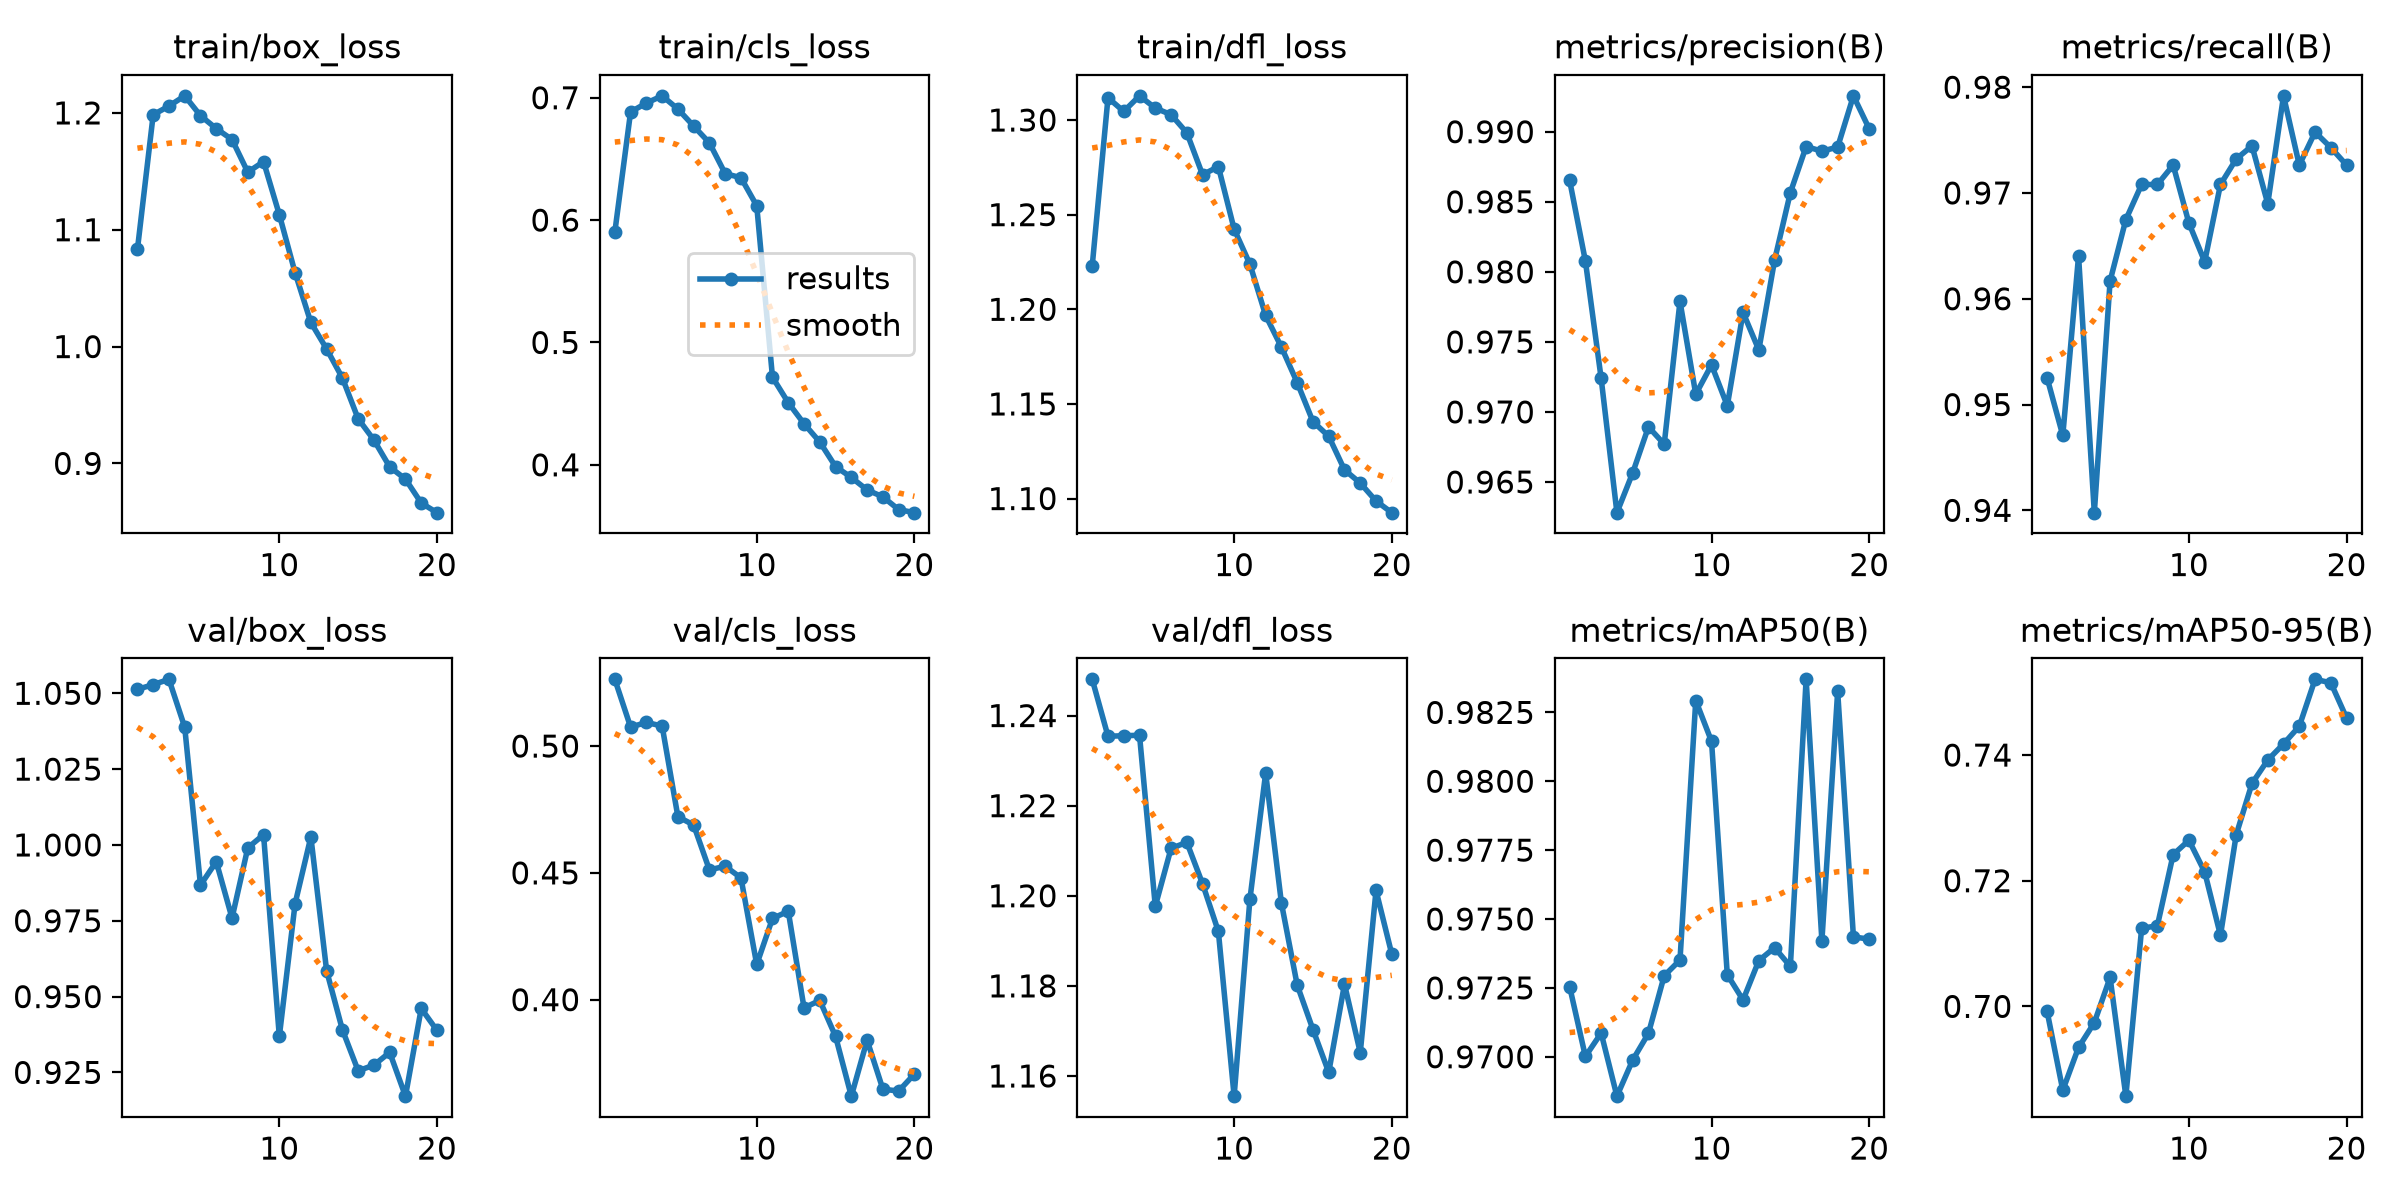
\includegraphics[width=0.58\textwidth]{training_curves.png}}
  \hfill
  \subfloat[Predictions on validation images.]{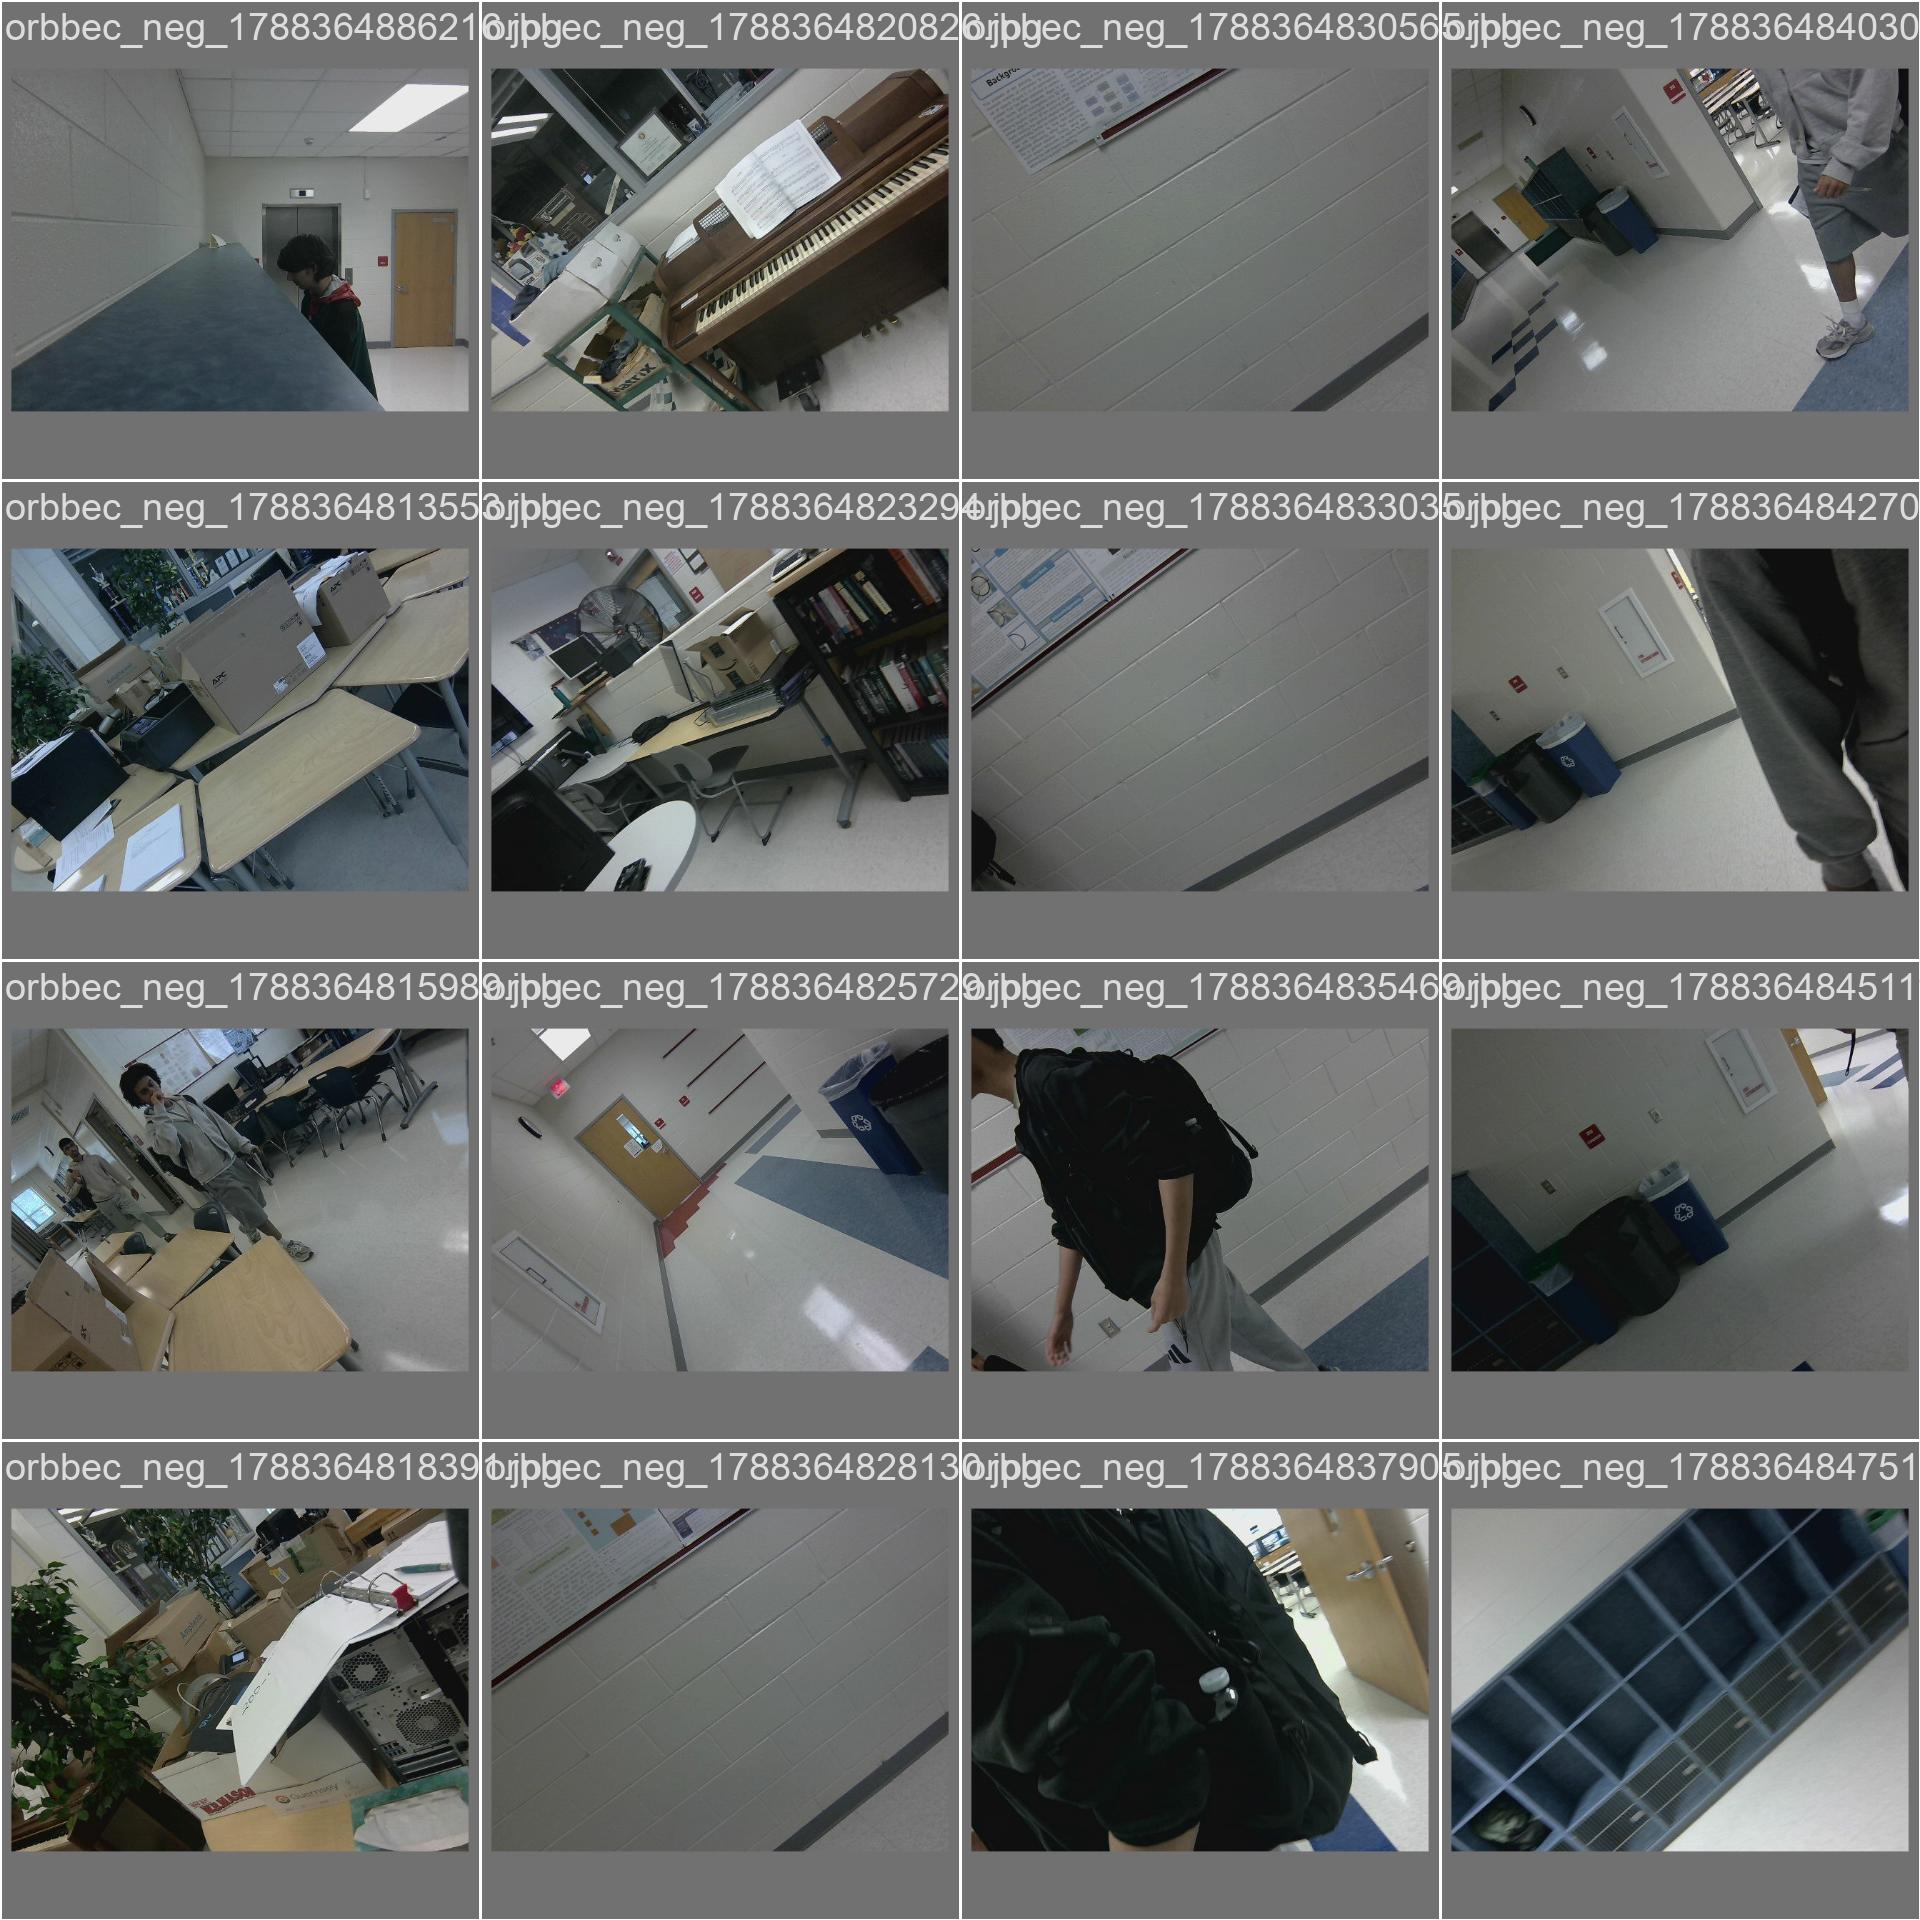
\includegraphics[width=0.40\textwidth]{val_predictions.jpg}}
  \caption{Detector training. Validation images are from the public collections.}
\end{figure}

\subsection*{Running it on the Jetson}

The perception node offered three inference backends: a TensorRT engine, OpenCV's CUDA
DNN, and OpenCV on the CPU. None of them could run on this Jetson. The image has no CUDA
toolkit or TensorRT installed, Ubuntu's OpenCV has no CUDA support, and OpenCV 4.5.4's
DNN module fails on the YOLOv8 head's reshape layer. I added a fourth backend on ONNX
Runtime \cite{onnxruntime}, which installs from a wheel and needs nothing from NVIDIA.
Through that path the 416-pixel model runs at 58\,ms per frame (17\,Hz) and the
640-pixel model at 124\,ms on the Orin's CPU with four threads. On 40 real validation
images the deployed 416 model found the car in every one.

Two guards were added in the node because a detector that is right 99\% of the time is
still dangerous when the 1\% is a hand at the lens reported as an opponent at 0.2\,m.
Detections implying a range under 0.8\,m or a box wider than 60\% of the frame are
dropped; inside that range the lidar owns the problem anyway. The confidence threshold
was raised from 0.35 to 0.5. The node is off by default in the car launch and enabled
with \texttt{use\_perception:=true}, since it costs a CPU core and only the head-to-head
agent uses it.

After the move to JetPack~7.2.1 (CUDA~13.2, TensorRT~10.16) the TensorRT path works, and
the engines are rebuilt on the car because they do not survive a TensorRT version change. The
640-pixel detector runs at 5.41\,ms mean and 6.04\,ms at the 99th percentile as an FP16 engine
(198 inferences per second), roughly 24 times faster than the ONNX Runtime CPU path above.

\section*{What the Architecture Buys}

Most of the individual pieces exist elsewhere. What matters here is that each one
removes a specific obstacle between this car and a learned policy.

\paragraph{Actions became measurable quantities.} The 2024 build could only send a PWM
pulse and hear nothing back. This car reports wheel speed at 20\,Hz, battery voltage and
temperatures, and accepts current commands directly. A logged demonstration is now a
triple of observation, action and outcome, all in physical units, and the same closed
loop is what let the current-mode launch fix the low-speed stall.

\paragraph{The camera is a motion sensor first.} The camera's most useful output is
its 200\,Hz inertial stream. It supplies the proprioceptive state a policy conditions on,
it de-skews the lidar so scans stay accurate at speed, and it gives the traction governor
a yaw rate. Vision is its second job.

\paragraph{One command channel for humans and policies.} Teleoperation, the joystick,
the Python client and any future policy server all publish the same
\texttt{sensor\_msgs/Joy}, behind the same watchdog. Swapping a human for a model changes
the sender, not the rest of the system, and the safety envelope does not care which one
is talking.

\paragraph{The dataset is not room-shaped.} Browser teleoperation over selectable
network modes means demonstrations can be collected by anyone with a link, in any space
the network reaches, on any device. That is the difference between a few hundred episodes
and a few thousand.

\paragraph{Firmware-level diagnosis, and firmware in the repository.} Reading and
writing the VESC's full configuration from the Jetson turned a silent failure into a
one-line diagnosis, and it makes the motor controller's state a versioned artifact
instead of something living in one laptop's settings.

\paragraph{Negatives from the deployed camera.} Public datasets tell a detector what a
car looks like. Only the target camera can tell it what the false alarms look like. Two
minutes of recording eliminated all 21 false detections, which is the small version of a
larger point: on-robot data beats more internet data.

\paragraph{Reproducibility as a deliverable.} The \texttt{hardware/} folder holds the
F1TENTH configuration overrides, the patch to the VESC driver, the udev rules that give
the gamepad, lidar, VESC and camera stable names and permissions, the VESC configuration
blobs and the tools that restore them, the network and launch scripts, and a runbook of
the failures above. This is what turns ``build a second car'' into a parts order, and a
second car is what makes any agent-to-agent work possible.

\section*{The Learned Policy on the Car}
\label{sec:policy}

\begin{figure}[H]
  \centering
  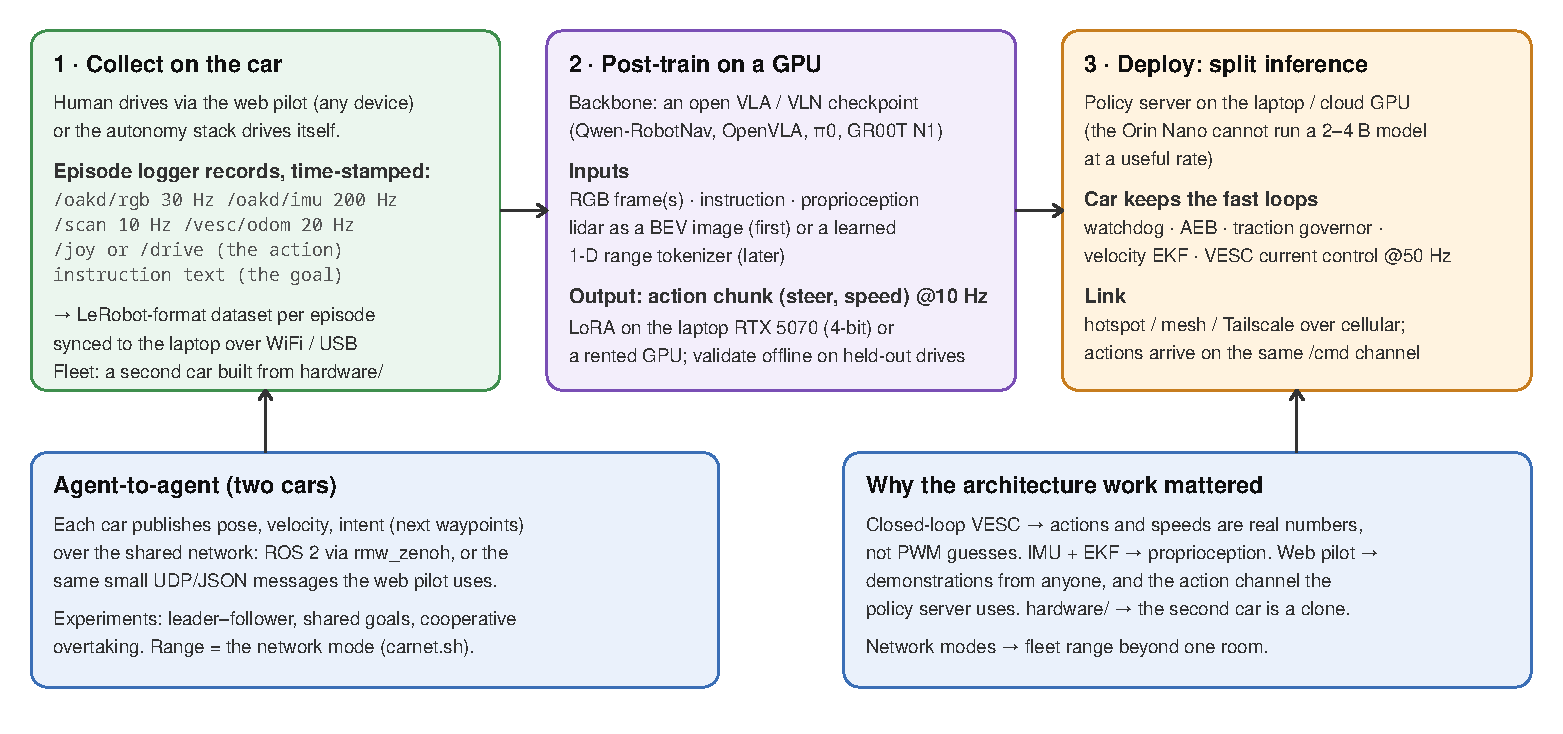
\includegraphics[width=\textwidth]{pivot_pipeline.pdf}
  \caption{The training pipeline. A goal-conditioned expert (A* route plus pure pursuit) drives
  in a ROS-free simulator; the student is trained on its demonstrations and on the states the
  student itself reaches (DAgger), exported to ONNX, and run on the car by
  \texttt{policy\_bridge} behind the same watchdog, emergency brake and command mux as every
  other driver.}
  \label{fig:pivot}
\end{figure}

The student takes four inputs every 100\,ms: the front camera frame resized to
96$\times$128, the lidar scan rasterised into a 96$\times$96 bird's-eye image covering 6\,m in
every direction, a 5-vector of proprioception, and the instruction text as hashed word tokens
(for example ``turn left, then go straight to the end and stop''). Two small convolutional
encoders, a bag-of-words embedding and a three-layer head (1.46\,M parameters in total) output
a speed and a steering angle. The expert is the simulator's goal-conditioned planner: A* on the
occupancy map inflated by the car's half-width, a pure-pursuit tracker, and a labeller that
turns the route into the instruction. \texttt{tools/sim\_generate.py} and
\texttt{ml/sim\_rollout.py} produce episodes in the car's own logging format, so the same
training code can later take real episodes.

On the car, \texttt{policy\_bridge} subscribes to the camera, the scan, odometry and the IMU,
runs the network with ONNX Runtime at 10\,Hz, clamps speed and steering, applies a forward-cone
emergency brake from the scan, and publishes on \texttt{/drive}, where \texttt{drive\_mux}
gives any human command priority for half a second.

\section*{On-Vehicle Inference}
\label{sec:inference}

Table~\ref{tab:latency} gives the measured cost of both networks on the Orin Nano in its 25\,W
mode, taken with the car on the bench and no actuator running. Pre-processing (resizing the
640$\times$360 camera frame and rasterising a 720-bin scan) costs 1.6\,ms per control tick.
The TensorRT FP16 student agrees with ONNX Runtime to within 0.0014\,m/s and 0.0004\,rad over
200 inputs.

\begin{table}[H]
  \centering
  \small
  \begin{tabular}{p{7.6cm} r r}
    \toprule
    Network and runtime & mean (ms) & p99 (ms) \\
    \midrule
    Student, ONNX Runtime CPU, 1 / 2 / 4 threads & 5.50 / 3.05 / 1.84 & 5.74 / 3.19 / 2.08 \\
    Student, TensorRT FP32 & 0.39 & 0.41 \\
    Student, TensorRT FP16 & 0.25 & 0.28 \\
    YOLOv8n-640 detector, TensorRT FP16 & 5.41 & 6.04 \\
    \midrule
    Student, TensorRT FP16, detector saturating the GPU & 1.70 & 2.77 \\
    Student, ONNX Runtime CPU, detector saturating the GPU & 1.68 & 1.77 \\
    Detector while sharing the GPU with the student & 5.75 & 7.86 \\
    \bottomrule
  \end{tabular}
  \caption{Inference latency on the Jetson Orin Nano Super (JetPack~7.2.1, 25\,W).}
  \label{tab:latency}
\end{table}

Both networks fit the 100\,ms control period many times over. The more useful result is the
contention row: with the detector keeping the GPU busy, the TensorRT student's mean latency grows
almost sevenfold and its tail more than that, while the CPU student is unaffected. For a network
this small the GPU buys nothing once another network is using it, so the student stays on the
CPU and the GPU belongs to the detector.

With the full stack running together on the bench (lidar, OAK-D, the policy, the TensorRT
detector and the raceline MPC, drive node off) the policy held 10.08\,Hz with control periods
between 89 and 104\,ms (standard deviation 3.8\,ms). All six CPU cores sat at 81--90\%, which is
the resource to watch, not the GPU. With the lidar and camera live and nothing able to move the
car, the corrected policy commanded 0.012\,rad of steering with 14.5\,m of clear space ahead.

\section*{A Closed-Loop Audit of the Learned Policy}
\label{sec:audit}

Before the work in this section, the student had a low offline validation error and had never
been run closed-loop through the same code that feeds it on the car. I wrote a ROS-free
evaluation (\texttt{ml/sim\_rollout.py}) that drives the policy in the simulator on a fixed,
seeded set of 150 goal tasks, 30 on each of five maps, one of which (\emph{uploadtest}) is
never used for training. It reports whether the car reaches within 0.5\,m of the goal without
touching a wall (success), whether it collides, and how much of the planned route it covers
(progress). Its inputs are built by \texttt{policy\_io.py}, the module that the car's bridge now
imports, so a number measured here is a number about the deployed pipeline. Table~\ref{tab:audit}
lists what it and the surrounding review found.

\begin{table}[H]
  \centering
  \small
  \begin{tabular}{p{4.2cm} p{10.3cm}}
    \toprule
    Problem & Effect and fix \\
    \midrule
    Action order swapped &
      The dataset stores (speed, steer); \texttt{policy\_bridge} unpacked (steer, speed). The
      predicted speed ($\approx$1.4\,m/s) became a steering command clamped to full lock and the
      predicted angle ($\approx$0) became the speed. Measured as deployed: 0\% success, 2.6\%
      progress; with the order fixed, \resBaseNomSucc\% and \resBaseNomProg\%. Fixed by one shared
      \texttt{policy\_io} module and an \texttt{action\_order} field in the ONNX metadata. The
      training log's two labels were swapped the same way, which hid it. \\
    Lossy lidar images &
      The bird's-eye raster was stored as mp4 video; only 47\% of true lidar pixels stayed above
      half intensity after decoding, while the car feeds the clean raster. Training now rebuilds
      it from the raw scan. \\
    Camera no longer fitted &
      Remote mode launched the removed Orbbec camera, so the bridge would have waited for images
      forever. The OAK-D Pro is now the default in launch, configuration and remote mode. \\
    Unobservable stops &
      The goal position is not in the observation, so ``stop here'' frames teach stopping at
      arbitrary places. They are dropped from training. \\
    Inertia problem &
      Given its own speed as input, the clone copied it (speed 0 in, speed 0 out) and never left
      the start line, the failure described by Codevilla et al.\ \cite{codevilla2019}. The speed
      and yaw-rate inputs are masked inside the exported model. \\
    NaN handling, shutdown &
      A NaN output was clamped to full lock before being checked; it is now zeroed first. The
      bridge sends an explicit zero command on exit, and the MPC no longer crashes on stop. \\
    \bottomrule
  \end{tabular}
  \caption{Problems found between training data and actuator.}
  \label{tab:audit}
\end{table}

\section*{Training for Closed Loop}
\label{sec:training}

Training data is 400 expert episodes (76\,817 frames) on four maps, generated in the
simulator with the car's lidar geometry and a 640$\times$480 rendered camera, and trained on
the laptop's RTX~5070. Three variants are compared, each with three seeds. \emph{BC, clean
data} is plain behaviour cloning on the new episodes. \emph{BC + augmentation} adds camera gain,
colour and noise augmentation, drops the camera frame entirely 30\% of the time, and randomly
removes up to 30\% of lidar beams (the RPLidar C1 returns about 19\% empty bins on the bench),
because the simulator's camera render will not look like the OAK-D. \emph{DAgger}
\cite{ross2011dagger} then lets the student drive, with the expert taking a tick with
probability 0.5, 0.25 and 0.1 in rounds 1--3, labels every state the student reaches with the
expert's action, and retrains on the aggregate.

\section*{Results}
\label{sec:results}

The platform measurements are in Table~\ref{tab:hw}; the closed-loop results of the learned
policy follow.

\begin{table}[H]
  \centering
  \small
  \begin{tabular}{p{5.2cm} p{9.6cm}}
    \toprule
    Quantity & Measured \\
    \midrule
    Lidar scan rate (\texttt{/scan}) & 10.0\,Hz, 720 bins, 16\,m \\
    Camera colour (\texttt{/oakd/rgb}) & 30\,Hz at 640$\times$480 (Orbbec, 2 Sept); OAK-D Pro 15.9--19.1\,Hz on 23 Sept \\
    Camera IMU (\texttt{/oakd/imu}) & 195--200\,Hz; gravity on body $+z$ = 9.75\,m/s$^2$ \\
    Velocity EKF (\texttt{/ekf/odom}) & 200\,Hz \\
    VESC telemetry / wheel odometry & 50\,Hz / 20\,Hz; 16.4\,V, MOSFETs 26--29\,\textdegree C, fault 0 \\
    Speed tracking on a stand & commanded 1500 / 3500 / 6000 / 9000 eRPM; measured 1472 / 3493 / 5986 / 9006 \\
    Gamepad path, manual stack & full throttle held 10\,000 eRPM at 3--4\,A; steering full range \\
    Detector & 58\,ms per frame at 416\,px on the CPU (2 Sept); 5.4\,ms at 640\,px in TensorRT (23 Sept) \\
    Web teleoperation & command round trip 1--2\,ms over the USB link; commands republished at 50\,Hz;
      steering follows to the servo limits; neutral within 250\,ms of the last packet \\
    \bottomrule
  \end{tabular}
  \caption{Hardware measurements, wheels off the ground or car stationary (2 and 23 September 2026).}
  \label{tab:hw}
\end{table}


\begin{table}[H]
  \centering
  \small
  \begin{tabular}{p{5.0cm} c r r r r}
    \toprule
    Policy & seeds & success \% [95\% CI] & collision \% & progress \% & unseen map \% \\
    \midrule
\csname @@input\endcsname results/table_nominal.tex
    \bottomrule
  \end{tabular}
  \caption{Closed-loop results in simulation on the same 150 seeded goal tasks (30 per map).
  Success = reached the goal without a collision. Confidence intervals are bootstrapped over
  the pooled episodes of all seeds. ``Unseen map'' is success on the map never used for
  training. The first row is the pre-9/23 student with the action-order bug fixed; as deployed
  it scored 0\%.}
  \label{tab:closedloop}
\end{table}

\begin{figure}[H]
  \centering
  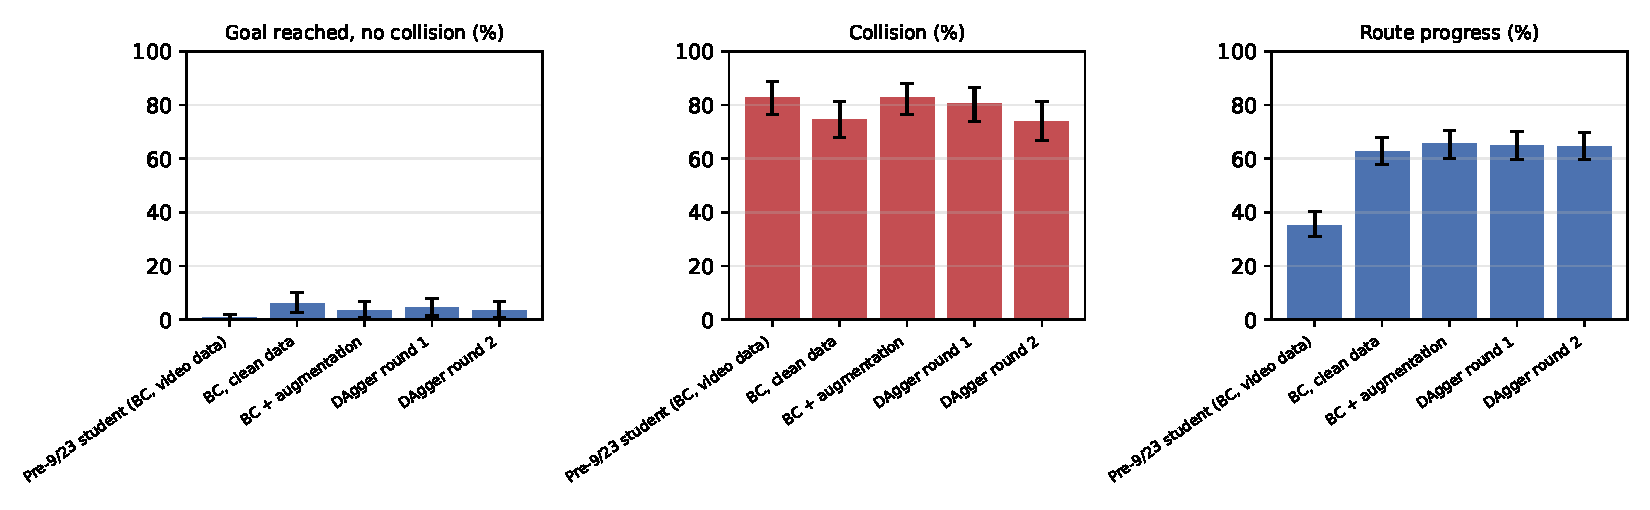
\includegraphics[width=\textwidth]{closed_loop_2026-09-23.pdf}
  \caption{Nominal closed-loop results (means with 95\% bootstrap intervals).}
  \label{fig:closedloop}
\end{figure}

\begin{table}[H]
  \centering
  \small
  \begin{tabular}{p{5.0cm} c c c c}
    \toprule
    Policy & nominal & lidar noise + 19\% dropout & camera shift & no camera \\
    \midrule
\csname @@input\endcsname results/table_robust.tex
    \bottomrule
  \end{tabular}
  \caption{Success \% / progress \% under simulated sensor degradation (sim-side proxies for
  the sim-to-real gap, not measurements on the car).}
  \label{tab:robust}
\end{table}

The interface fixes are the large effect: with clean data and the inertia problem removed,
the policy covers \resBcNomProg\% of the route on average, against \resBaseNomProg\% for the
old student even after its action order is corrected, and 2.6\% as it was deployed. Goal
success is a different matter. Without the goal in its observation, a memoryless policy must
infer from the instruction and the scene alone where to turn and where the route ends, and it
still leaves the route or touches a wall on most long tasks. Augmentation did not raise nominal
success, though it made the policy indifferent to losing the camera entirely. Three rounds of
DAgger left success at \resDgthreeNomSucc\% with \resDgthreeNomColl\% collisions, so on this task
the missing information (where the goal is, and which turns have already been taken) matters
more than the distribution shift that DAgger corrects. These are the
numbers to beat, not a claim that the policy is ready to race.

An input ablation (one seed, clean-data behaviour cloning, the removed input zeroed inside the
exported network) asks which sensor the policy relies on: with the lidar raster alone it reached
\resAbllidNomSucc\% success and \resAbllidNomProg\% progress, with the camera alone
\resAblcamNomSucc\% and \resAblcamNomProg\%, against \resBcNomSucc\% and \resBcNomProg\% with
both (three-seed mean). Because the simulator's camera is a render, this says what the policy
can do with each input in simulation, not which one will transfer better.

\section*{Software Platform: Ubuntu 26.04 and ROS 2 Lyrical}
\label{sec:lyrical}

The car runs JetPack~7.2.1 on Ubuntu~24.04 with ROS~2 Jazzy. NVIDIA's JetPack~7 is built on
Ubuntu~24.04 \cite{jetpack}, the installed TensorRT Python binding requires Python~3.12 while
Ubuntu~26.04 ships 3.14, and the SD card has one root partition with no fallback, so an in-place
upgrade four days before a competition is not justified. Instead, an Ubuntu~26.04 image with ROS~2
Lyrical \cite{roslyrical} is built on the car itself (\texttt{docker/lyrical/Dockerfile}); the car
has no internet of its own, so packages come through a small allowlisted proxy on the laptop over
an SSH reverse tunnel. Inside it the package builds with \texttt{colcon}, 48 of its 49 Python
modules import (the exception needs the legacy \texttt{gym} used only by the simulator bridge),
and all 149 unit tests pass, the same count as on the host. A native upgrade plan, starting from a
cloned SD card so the original remains the rollback, is in \texttt{docs/ubuntu26\_native\_plan.md}.
One finding from this work applies to everything: the car has no real-time clock battery or time
source and boots with a stale date, which breaks certificate and package-list validation.

\section*{Limitations}

Every closed-loop number in this report is from simulation. The simulator's camera is a
distance-shaded raycast render, so the camera encoder has never been trained on a real image;
the robustness table uses simple sim-side perturbations as proxies, not the real sensor. The
bicycle model has no tyre slip and a point-sized car for collisions. The hardware measurements
were taken on the bench: the learned policy has not driven the floor, and the concurrency run had
no localisation, so the MPC was not solving. Goal success remains low; the result of this work is
a deployment path that can be trusted and measured, not a finished policy.

\section*{Next Steps}

Move the student to a task its inputs can support, lap following on a race line with the MPC as
expert, which is also the competition task. Collect real episodes with the OAK-D and the C1
through \texttt{episode\_logger}, measure the offline sim-to-real gap on them, and then run the
student on the floor at 0.6\,m/s behind the emergency brake and the human-priority mux. Repeat
the concurrency test with localisation running, and find what is using the CPU. Fix the clock.

Two warnings for whoever picks this up remain from the platform work. Keep the battery connector
keyed or marked: the VESC dies instantly on reversed leads. And read
\texttt{hardware/RUNBOOK.md} before touching the VESC's application settings, because the shared
PPM/servo pin will look like a dead motor controller to anyone who does not know about it.

\section*{Acknowledgments}

[To be completed: research teacher, lab, teammates who built the chassis and the
simulation stack, and whoever soldered the phase leads at three in the morning.]

\printrefs

\end{document}
